\documentclass{article}
\usepackage[english]{babel}
\usepackage[T1]{fontenc}
\usepackage[hidelinks]{hyperref}
\usepackage{multicol}
\usepackage{multirow}
\usepackage{tabularx}
\usepackage{graphicx}
\usepackage{float}
\hypersetup{
    colorlinks=true,
    linkcolor=blue,
    filecolor=magenta,      
    urlcolor=blue,
    pdfpagemode=FullScreen,
    }

%%%%%%%%%%%%%%%%%%%%%%%%%%%%%%%%%%%%%%%%%%%%%%%%%%%%%%%%%%%%%%%
\begin{document}
\section{Preliminaries}
\large
First, download the figures from the web by right clicking and selecting "Save Link As".
\bigskip
\begin{itemize}
\item \url{https://raw.github.com/rjp0i/latex-intro/master/en/gerbil.jpg}

\item \url{https://raw.github.com/rjp0i/latex-intro/master/en/lithium.png}

\end{itemize}


\medskip

Then upload the images into this Overleaf Project. You will then need to recompile this project in Overleaf, so that the images are added to this PDF (check the next page to see if an image appears).
\bigskip

\bigskip


The PDF for this entire workshop can be found here:


\item \url{https://raw.github.com/rjp0i/latex-intro/master/en/latex-fig-tab.pdf}



\clearpage
%%%%%%%%%%%%%%%%%%%%%%%%%%%%%%%%%%%%%%%%%%%%%%%%%%%%%%%%%%%%%%%%
\section{First Figure}

Here is a figure, with no caption
\medskip

{\bf Your Turn: Try changing the width of the figure}

\begin{figure}
\centering   %centers the figure (horizontally) on the page
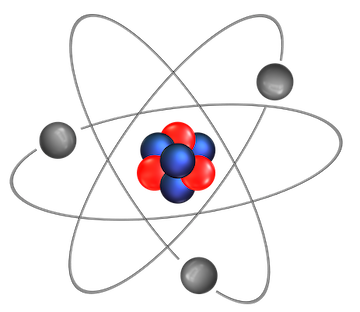
\includegraphics[width=1.5in]{lithium.png} %sets the figure width to 1.5in
\end{figure}
\clearpage
%%%%%%%%%%%%%%%%%%%%%%%%%%%%%%%%%%%%%%%%%%%%%%%%%%%%%%%%%%%%%%%
\section{Captioning a Figure}
Here is a figure, with a caption

\begin{figure}
\centering
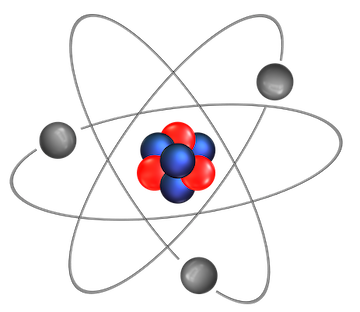
\includegraphics[scale=0.5]{lithium.png} %scales the figure down to 50% of the original size
\caption{This is Lithium (${}^{6}$Li)}
\end{figure}
\clearpage
%%%%%%%%%%%%%%%%%%%%%%%%%%%%%%%%%%%%%%%%%%%%%%%%%%%%%%%%%%%%%%%
\section{Labeling a Figure}
Figure \ref{fig:gerbil} shows the automatic numbering of figures (both in the caption, as well as here, in the text of the document itself.

{\bf Your turn: }
\begin{figure}
\centering

\includegraphics[
  width=0.5\textwidth]{gerbil}
\caption{\label{fig:gerbil}Aww\ldots.}
\end{figure}
\clearpage
%%%%%%%%%%%%%%%%%%%%%%%%%%%%%%%%%%%%%%%%%%%%%%%%%%%%%%%%%%%%%%%
\section{Placing a Figure}
Figure \ref{fig:gerbil2}, shown below, shows how one can position a figure on a page.

{\bf Your Turn: Try changing the placement of the figure, using the options h, t, b, p, !, and H}
\begin{figure}[h]
\centering

\includegraphics[width=0.5\textwidth]{gerbil}
\caption{\label{fig:gerbil2}Aww\ldots.}
\end{figure}
\clearpage
%%%%%%%%%%%%%%%%%%%%%%%%%%%%%%%%%%%%%%%%%%%%%%%%%%%%%%%%%%%%%%%

\section{Simple Tables}

A very basic table
\bigskip

\begin{tabular}{lrr}
Item   & Qty & Unit \$ \\
Widget & 1   & 199.99  \\
Gadget & 2   & 399.99  \\
Cable  & 3   & 19.99   \\
\end{tabular}
\bigskip

{\bf Your Turn:}
Try changing the alignment of the columns.

{\bf Your Turn again (after next slide):}
Try adding horizontal and vertical lines to the table.

\clearpage
%%%%%%%%%%%%%%%%%%%%%%%%%%%%%%%%%%%%%%%%%%%%%%%%%%%%%%%%%%%%%%%
\section{Lining up using @-expressions}

\begin{tabular}{r@{.}l} \hline
  3   & 14159 \\
  16  & 2     \\
  123 & 456   \\  \hline
\end{tabular}
\bigskip

{\bf Your turn:}
\begin{enumerate}
\item What happens if you change the alignment for the two columns from right, left to left, right? 
\item Try changing the content of the @-expression from a decimal point to something else
\end{enumerate}
\clearpage
%%%%%%%%%%%%%%%%%%%%%%%%%%%%%%%%%%%%%%%%%%%%%%%%%%%%%%%%%%%%%%%
 \section{multicolumn  and multirow}


\begin{tabular}{|l|l|r|} \hline
  \multicolumn{2}{|c|}{Item} & \multirow{2}{*}{Price (\$)}\\ \cline{1-2}
  Animal & Description &  \\ \hline
  Gnat  & per gram & 13.65 \\
        & each     &  0.01 \\
  Gnu   & stuffed  & 92.50 \\
  Emu   & stuffed  & 33.33 \\
  Armadillo & frozen & 8.99 \\ \hline
 \end{tabular}
  
 \bigskip
  
{\bf Your turn:} 
\begin{enumerate}
\item What happens if you change Gnat to %${\backslash}$multirow\{2\}\{*\}\{Gnat\}?
 % \multirow{2}{*}{Gnat}
\item What happens if you replace the cline 1-2 command with an hline command?  
\end{enumerate}
\clearpage
%%%%%%%%%%%%%%%%%%%%%%%%%%%%%%%%%%%%%%%%%%%%%%%%%%%%%%%%%%%%%%%
 \section{Positioning, Captioning, and Labeling a Table}

\begin{table}[b]
\centering
\begin{tabular}{|l|l|r|} \hline
  \multicolumn{2}{|c|}{Item} & \multirow{2}{*}{Price (\$)}\\ \cline{1-2}
  Animal & Description &  \\ \hline
  Gnat  & per gram & 13.65 \\
        & each     &  0.01 \\
  Gnu   & stuffed  & 92.50 \\
  Emu   & stuffed  & 33.33 \\
  Armadillo & frozen & 8.99 \\ \hline
 \end{tabular}
 \caption{\label{tab:prices}Wholesale Prices}
 \end{table}
  
 \bigskip
  
{\bf Your turn:} 
\begin{enumerate}
\item Refer to the table in the text
\item Move the location of the table with the positioning parameter
\end{enumerate}
\clearpage
\end{document}
